\Chapter{Angular2 implementáció}

CRUD műveletek: a műveletek megvalósításához szükséges funkciókat a szerviz tartalmazza, ebben az esetben a FighterService.

\begin{cpp}
@Injectable()
export class FighterService {
  constructor(private http: Http) { }
  getAllFighters() {
    return new Promise((resolve, reject) => {
      this.http.get('/fighter')
        .map(res => res.json())
        .subscribe(res => {
          resolve(res);
        }, (err) => {
          reject(err);
        });
    });  }  }
\end{cpp}

A getAllFighters() GET kérést küld a szervernek. Ennek a függvénynek a segítségével kérhetők le az eltárolt harcosok és adataik.
Egy harcos adatainak frissítésére szolgál az "updateFighter()" függvény:

\begin{cpp}
updateFighter(id, data) {
    return new Promise((resolve, reject) => {
        this.http.put('/fighter/'+id, data)
          .map(res => res.json())
          .subscribe(res => {
            resolve(res);
          }, (err) => {
            reject(err);
          });
    });
  }
\end{cpp}

A HTML oldalakat külön komponensek vezérlik.

Ezeket a komponenseket az "ng g component komponensnév" paranccsal lehet létrehozni, ami automatikusan legenerálja a szükséges fájlokat és hozzáadja az új komponenst az "app.module.ts" fájlhoz.

\begin{cpp}
@Component({
  selector: 'app-fighter',
  templateUrl: './fighter.component.html',
  styleUrls: ['./fighter.component.css']
})
export class FighterComponent implements OnInit {
  fighters: any;
  constructor(private fighterService: FighterService) { }
  ngOnInit() {
    this.getFighterList();
  }
  getFighterList() {
    this.fighterService.getAllFighters().then((res) => {
      this.fighters = res;
    }, (err) => {
      console.log(err);
    });}}
\end{cpp}

A "fighters" oldal, ami a harcosok megjelenítésére szolgál egy komponens, a hozzátartozó template-t a "templateUrl" kifejezéssel tudjuk megadni. A kinézetét a megfelelő nevű, .css kiterjesztésű fájl tartalmazza, amelyet a "styleUrls" kifejezéssel adhatunk meg.

Ez az oldal a "getFighterList()" nevű függvény használatával kéri le a szerveren tárolt harcosokat.

A harcosok táblázatának keresőmezővel történő szűréséhez egy úgynevezett "pipe"-ra van szükségünk:

\begin{cpp}
export class FilterPipe implements PipeTransform {
  transform(fighters: any, search: any): any {
    if (search === undefined) return fighters;
    return fighters.filter(function(fighter){
    	return fighter.name.includes(search);  })}}
\end{cpp}

Ezenkívül szükség van még egy kereső mezőre: 

\begin{cpp}
<input type="text" [(ngModel)]="search" 
placeholder="Search fighters..."/>
\end{cpp}

Használata a "| filter:szűrőmező neve" paranccsal lehetséges:

\begin{cpp}
<tbody>
      <tr *ngFor="let fighter of fighters | filter:search">
        <td>{{ fighter.name }}</td>
        <td>{{ fighter.nickname }}</td>
      </tr>
    </tbody>
\end{cpp}

Továbbá szükség van egy "import"-ra, amelyet az app.module.ts fájlhoz kell hozzáadnunk:

\begin{cpp}
import { FilterPipe } from './filter.pipe';
\end{cpp}

Majd ugyanebben a fájlban az @NgModule "declarations" részéhez hozzá kell adni a FilterPipe osztályt:

\begin{cpp}
@NgModule({
  declarations: [
    AppComponent,
    HomeComponent,
    FighterComponent,
    FilterPipe
\end{cpp}

\Section{Routing}

A routing-hoz szükség van a

\begin{cpp}
import { RouterModule } from '@angular/router';
\end{cpp}

sorra, amit az "app.module.ts" nevű fájlban kell megadnunk.
Továbbá szükséges még az "app.component.html" fájlban a <router-outlet></router-outlet> tag-ok megadása.

Route-k (útvonalak) létrehozása az "app.routes.ts" fájlban történik.

\begin{cpp}
export const ROUTES: Routes = [
  { path: ' ', component: HomeComponent },
  { path: 'fighters', component: FighterComponent },
  { path: '**', redirectTo: ' ' }
];
\end{cpp}

Ezenkívül szükséges a következő "import" megadása az "app.module.ts" fájlban:

\begin{cpp}
import { ROUTES } from './app.routes'; 
\end{cpp}

A lapok közötti navigálás linkekkel történik.
A "/fighter-create" oldalról a "/fighters" oldalra való visszalépés esetén:

\begin{cpp}
<a [routerLink]="['/fighters']">Go back</a>
\end{cpp}

\Section{Form validáció}

A form validációnál a "disabled"-re (letiltott) állítottam a "Submit" gombot:

\begin{cpp}
<button type="submit" class="btn btn-success" 
[disabled]="!fighterForm.form.valid">Submit</button>
\end{cpp}

Így ha a "fighterForm" nevű űrlap (form) nem valid, akkor a "Submit" gomb ki van kapcsolva.

Mezők validálása az Angular 2 által biztosított direktívákkal történik:

\begin{cpp}
<form (ngSubmit)="saveFighter()" #fighterForm="ngForm">
\end{cpp}

A form fejlécében meg kell adni a form nevét, ez esetben "fighterForm".

Majd a "Submit" gomb letiltása a [disabled]="!fighterForm.form.valid" sor "Submit" gombhoz való hozzáadásával érhető el.

\begin{cpp}
<button type="submit" class="btn btn-success" 
[disabled]="!fighterForm.form.valid">Submit</button>
\end{cpp}

A name mező validálásához meg kell adni a kívánt direktívákat, ebben az esetben, a mező kitöltésekor minimum három karakter hosszúságú nevet kell beírnia a felhasználónak. (minlength=”3”)

A "required" jelző pedig a mező kitöltését követeli meg a felhasználótól:

\begin{cpp}
<label for="name">Name*</label>
<input type="text" class="form-control" [(ngModel)]="fighter.name" 
name="name" id="name" #name="ngModel" required minlength="3">
<div *ngIf="name.errors && (name.dirty || name.touched)" 
	class="alert alert-danger">
	<div [hidden]="!name.errors.required">
    	Name is required!
    </div>
    <div [hidden]="!name.errors.minlength">
    	Name must be at least 3 characters long.
    </div>
</div>
\end{cpp}

Ha a "name" mező hibás és már írtak bele vagy csak belekattintottak, akkor a mező alatt megjelenítődik az épp aktuális hibaüzenet.

A "record" mező validálásához "pattern"-t kell hozzáadni a mezőhöz:

\begin{cpp}
<label for="record">Record*</label>
<input type="text" class="form-control" [(ngModel)]="fighter.record" 
name="record" id="record" #record="ngModel" 
pattern="[0-9]{1,2}-[0-9]{1,2}-[0-9]{1,2}" required>
<div *ngIf="record.errors && (record.dirty || record.touched)" 
class="alert alert-danger">
<div [hidden]="!record.errors.required">
	Record is required!</div>
<div [hidden]="!record.errors.pattern">The record must be in 
Wins-Draws-Losses form.</div></div>
\end{cpp}

Ha a beírt adatok nem egyeznek meg a "pattern"-nel, akkor a felhasználó a "The record must be in wins-draws-losses form" hibaüzenetet kapja.

A harcos avatarjának image\_url mezőben megadott URL linkhez tartozó validációjánál itt is a pattern="https?://.+" direktívát kell a beviteli mezőhöz hozzáadni. Ezt követően, ha a felhasználó az "Image URL" linket nem a megfelelő formában adja meg, akkor az "Image URL must be valid!" hibaüzenetet kapja.
\newpage

\Section{Projekt struktúra}

\begin{figure}[htb]
\centering
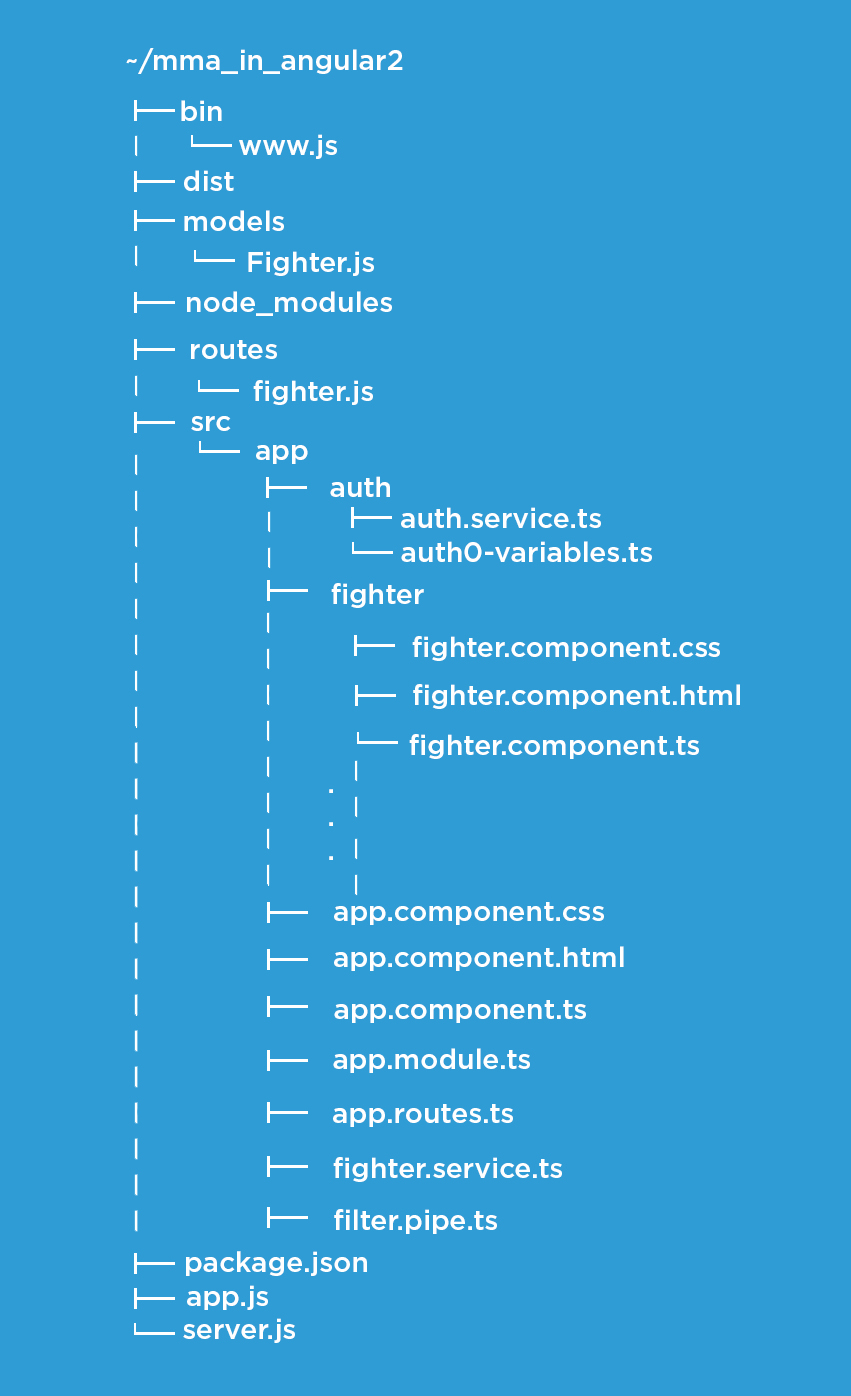
\includegraphics[scale=0.7]{kepek/mma_in_angular2.jpeg}
\caption{Az Angular 2 projekt struktúrája}
\label{fig:angular2_structure}
\end{figure}

A (\ref{fig:angular2_structure}. ábra) az Angular 2 webalkalmazáshoz tartozó projekt felépítését mutatja be. A különböző komponensek jól elkülöníthetők egymástól, mindegyik esetében megtalálhatók a .css, a .html és .ts kiterjesztésű fájlok. A .ts (TypeScript) fájlban vannak definiálva a különböző függvények, konstruktorok, és metódusok. A .html a felhasználó elé táruló weblap kinézetéért felel, a .css fájl pedig a megjelenített .html oldal stílusát adja meg. \cite{Angular 2 könyv} \cite{Angular 2 oldal} 